\chapter{Implementation
    \label{chapter:implementation}}

This chapter discribs the tools, methods and reasons for the from of implementation.
As sad due to early test CLIP and TinyCLIP are used as models.

\section{Model acquisition}

The CLIP models are taken from the official CLIP Github repo \cite{clipgit}.
The TinyCLIP models are taken from the official TinyCLIP Github repo \cite{tinyclipgit}.
There is also the posibility to take models from HuggingFace \cite{huggingface}.
The problem with HuggingFace is that the model cant be split into image and text encoder.

\section{Model translation}
The models were first split into image and text encoder.
The image encoder then gets translated to a onnx graph and afterwards simplified.
This onnx graph then is translated by the \acrshort{dfc} to \acrshort{har} and \acrshort{hef} files.

\begin{figure}
    \centering
    \subfloat[End of CLIP ResNet50x4 vision encoder Onnx graph acquired though official CLIP]{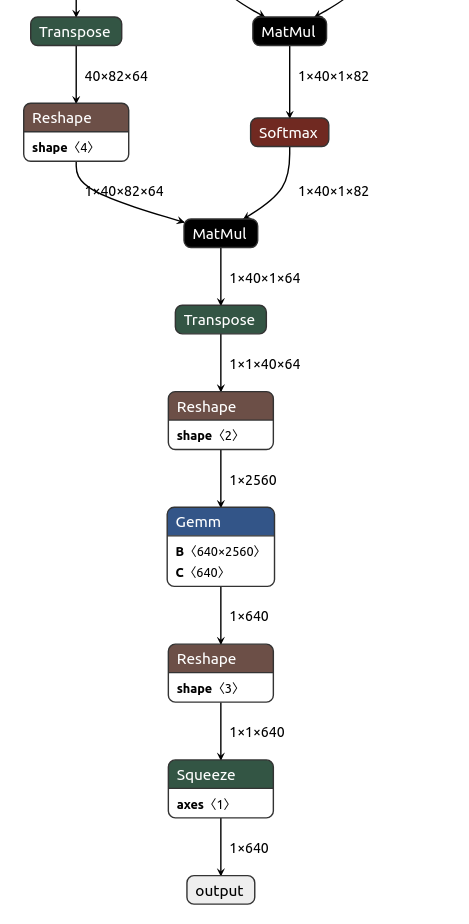
\includegraphics[width=0.4\textwidth]{Images/Implementation/ClipRes50x4.png}\label{fig:implementation:clipres50x4}}
    \qquad
    \subfloat[End of CLIP ResNet 50x4 vision encoder Onnx graph sendt by Hailo]{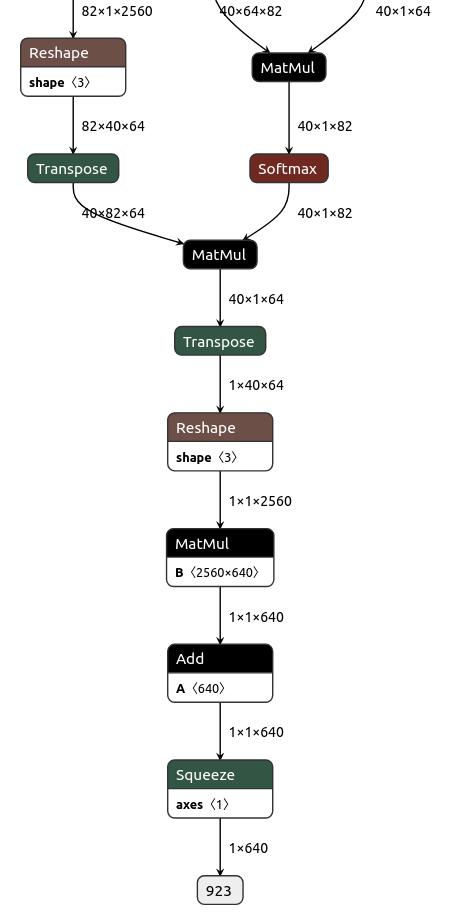
\includegraphics[width=0.4\textwidth]{Images/Implementation/HailoClipRes50x4.png}\label{fig:implementation:hailoclipres50x4}}
    \caption{Comparison of CLIP ResNet 50x4 vision encoder Onnx graph (a) from official CLIP and (b) from Hailo}
    \label{fig:implementation:compareRN50x4}
\end{figure}

In that step lays the first big problem of the project.
As described in \cref{section:dfc} the dfc is unable to compile transformers.
To be precise a transpose block at the end of every self attention layer is were the problems lay.
The dfc swaps dimensions and takes together the last 2 dimensions.
In the ResNet which is acquired though the offical code (see \cref{fig:implementation:clipres50x4})one can see that the transpose block after the MatMul block swaps a second and the third dimension.
This leads to a compilation error because the \acrshort{dfc} already combined the last 2 dimensions.
This error doesnt occure when the model given by Hailo is compiled.
In \cref{fig:implementation:hailoclipres50x4} the maximum of dimensions is 3.

To work around this problem the last part of the onnx graph is cut off.
To cut the graph \cite{onnxmodifier} is used.
The cut off blocks are implemented as postprocessing.

After compilation the graph can again be visualized with a tool name profiler from hailo.
In \cref{fig:implementation:compareRN50x4qunathar} the compiled model with the cutoff end is visualized.
in the fogure the combination of the last dimensions can be seen.
\begin{figure}
    \centering
    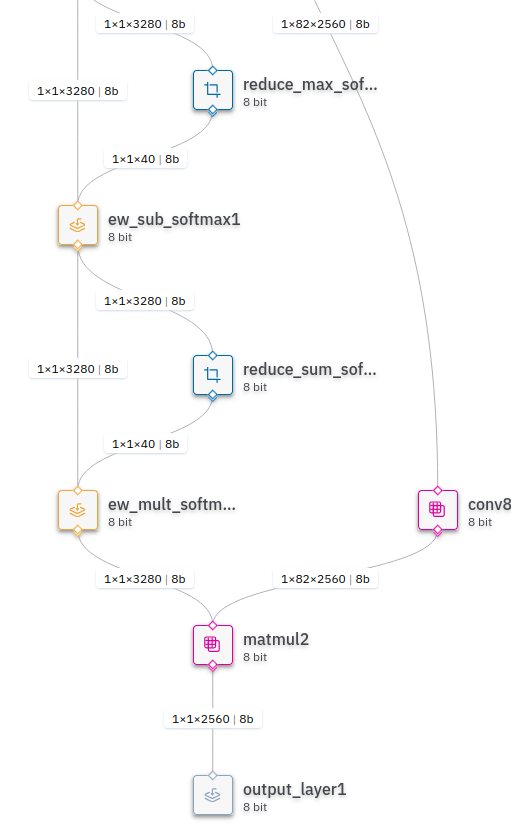
\includegraphics[width=0.4\textwidth]{Images/Implementation/ClipRes50x4_qunat_Har.png}
    \caption{Output of the \acrshort{dfc} from compiling the modified onnx graph of the ResNet50x4.}
    \label{fig:implementation:compareRN50x4qunathar}
\end{figure}

\section{Inference}

\subsection{Preprocessing}

Clip preprocessor.
split Images.

\section{Measurments}